\section{Sistemas de Reconhecimento de Locutor}
\label{sec:speaker-recognition-systems}

\contentscurrent

\subsection{Identificação}

\begin{frame}
\frametitle{Identificação}
\begin{description}
    \item[Modelagem] Para cada locutor $\mathcal{S}_j \in \boldsymbol{\mathcal{S}}$
    \begin{itemize}
        \item Extrair $\boldsymbol{X}_k$ dos sinais $\boldsymbol{Y}_k$ falados por $\mathcal{S}_j$
        \item Treinar um $\lambda_j$ para cada $\mathcal{S}_j$ através dos $\boldsymbol{X}_k$
    \end{itemize}
    \item[Teste] Para um locutor desconhecido $\mathcal{S}$
    \begin{itemize}
        \item Extrair $\boldsymbol{X}$ do sinal $\boldsymbol{Y}$ falado por $\mathcal{S}$
        \item $i = \arg_j\max\postpdf{\boldsymbol{X}}{\lambda_j} \implies \mathcal{S} \gets \mathcal{S}_i$
    \end{itemize}
\end{description}

\begin{figure}[ht]
    \centering
    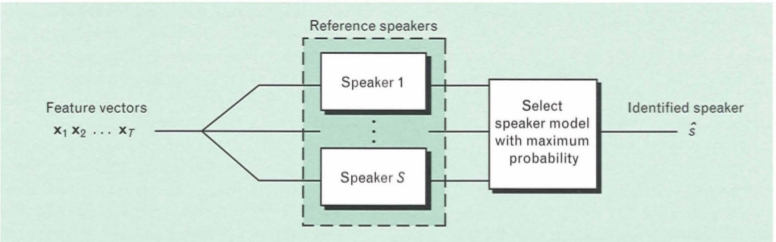
\includegraphics[width=0.75\textwidth]{speaker-identification}
\end{figure}
\end{frame}

\subsection{Verificação}

\begin{frame}
\frametitle{Verificação}
\begin{description}
    \item[Modelagem] Para todos os $\mathcal{S}_j \in \boldsymbol{\mathcal{S}}$
    \begin{itemize}
        \item Extrair $\boldsymbol{X}_k$ dos sinais $\boldsymbol{Y}_k$ falados por cada $\mathcal{S}_j$
        \item Treinar um $\lambda_{bkg}$ através dos $\boldsymbol{X}_k$ de todos os $\mathcal{S}_j$
        \item Modelar um $\lambda_j$ para cada $\mathcal{S}_j$
    \end{itemize}
    \item[Teste] $\mathcal{S}$ diz ser $\mathcal{S}_C \in \boldsymbol{\mathcal{S}}$
    \begin{itemize}
        \item Extrair $\boldsymbol{X}$ do sinal $\boldsymbol{Y}$ falado por $\mathcal{S}_C$
        \item $\Lambda(\boldsymbol{X}) = \log p(\boldsymbol{X}|\lambda_{C}) - \log p(\boldsymbol{X}|\lambda_{bkg})$
        \item $\Lambda(\boldsymbol{X}) \geq \theta \implies aceita$
    \end{itemize}
\end{description}

\begin{figure}[ht]
    \centering
    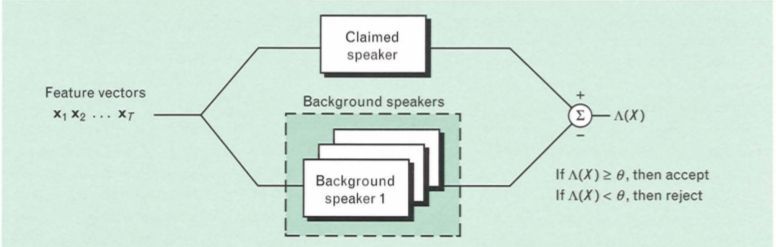
\includegraphics[width=0.75\textwidth]{speaker-verification}
\end{figure}
\end{frame}